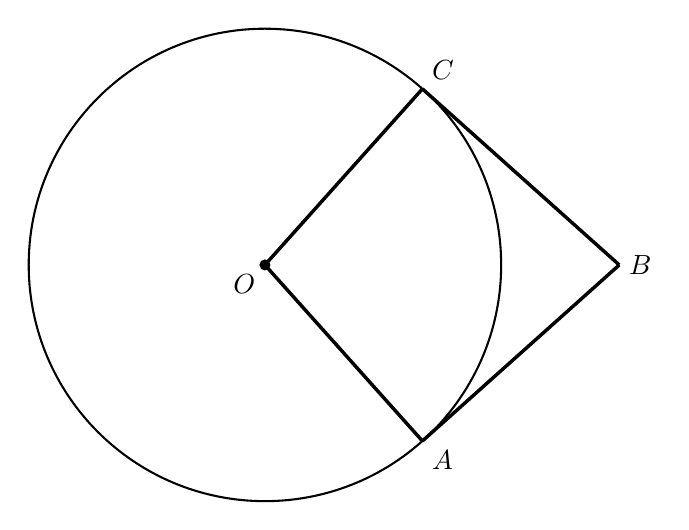
\begin{tikzpicture}[baseline=0]
    % Circle parameters
    \def\r{3} % radius of the circle
    \def\q{4.5} % distance from the center to the external point
    \def\x{{\r^2/\q}} % x coordinate of the point of tangency
    \def\y{{\r*sqrt(\q^2-\r^2)/\q}} % y coordinate of the point of tangency

    % Draw the circle with radius 3
    \draw[line width=.75pt] (0,0) circle (\r);

    % Define points
    \coordinate (O) at (0,0); % Center of the circle
    \coordinate (P) at (\q,0); % External point
    \coordinate (T1) at (\x,\y); % Tangent point 1
    \coordinate (T2) at (\x,-\y); % Tangent point 2

    % Draw radii and tangent lines
    \draw[line width=1.25pt] (O) -- (T1);
    \draw[line width=1.25pt] (O) -- (T2);
    \draw[line width=1.25pt] (P) -- (T1);
    \draw[line width=1.25pt] (P) -- (T2);

    % Mark the center of the circle with a dot
    \fill (O) circle (2pt);
    \node at (O) [below left] {$O$};

    % Label the external point and tangent points
    \node at (P) [right] {$B$};
    \node at (T1) [above right] {$C$};
    \node at (T2) [below right] {$A$};
\end{tikzpicture}